\documentclass{../../note}

\usepackage{amsthm}
\usepackage{pgfplots}
\pgfplotsset{compat=1.18}
\newtheorem{example}{Example}
\usepackage{xcolor} % For colored text
\usepackage{tikz}
\usetikzlibrary{shapes,arrows,positioning,fit,calc,matrix}
\usepackage{algorithm}
\usepackage{algpseudocode}
\usepackage{listings}
\lstset{
  basicstyle=\ttfamily\small,
  keywordstyle=\color{blue},
  commentstyle=\color{green!60!black},
  stringstyle=\color{purple},
  numbers=left,
  numberstyle=\tiny,
  numbersep=5pt,
  breaklines=true,
  frame=single,
}

\title{数据结构 03}
\author{isomo}

\begin{document}

\maketitle

考纲内容:

\begin{itemize}

  \item \textbf{树和二叉树: }
    树的基本概念,二叉树的概念、性质和存储结构,二叉树的遍历,线索二叉树,哈夫曼树。

  \item \textbf{图: }
  图的基本概念与存储结构,图的遍历算法,最小生成树(Prim 和 Kruskal 算法),最短路径(Dijkstra 算法)。
\end{itemize}

\section{树和二叉树}

\subsection{树的基本概念}

\subsubsection{定义}
\textcolor{red}{树(Tree)是 $n$ ($n \geq 0$) 个结点的有限集。当 $n=0$ 时称为空树。在任意一棵非空树中,有且仅有一个特定的称为根(Root)的结点,剩余结点可分为 $m$ ($m \geq 0$) 个互不相交的有限集,每个集合本身又是一棵树,称为原树的子树(Subtree)。}

\subsubsection{术语}
\begin{itemize}
\item \textbf{结点的度}:结点拥有的子树个数
\item \textbf{树的度}:树内各结点的度的最大值
\item \textbf{叶子结点}:度为 0 的结点
\item \textbf{分支结点}:度不为 0 的结点
\item \textbf{结点的层次}:从根开始定义,根为第 1 层,根的孩子为第 2 层
\item \textbf{树的高度/深度}:树中结点的最大层次
\item \textbf{森林}:$m$ ($m \geq 0$) 棵互不相交的树的集合
\end{itemize}

\subsubsection{树的表示方法}
\begin{enumerate}
\item \textbf{双亲表示法}:使用数组存储,每个结点中附设一个指向其双亲的指针
\item \textbf{孩子表示法}:每个结点有多个指针指向其孩子结点
\item \textbf{孩子兄弟表示法}:每个结点设两个指针,分别指向第一个孩子和下一个兄弟
\end{enumerate}

\subsection{二叉树的概念与性质}

\subsubsection{定义}
\textcolor{red}{二叉树(Binary Tree)是一种树形结构,每个结点最多有两个子树,分别称为左子树和右子树。二叉树是有序树,其左右子树不能互换。}

\subsubsection{特殊二叉树}
\begin{itemize}
\item \textbf{满二叉树}:所有分支结点都有左子树和右子树,且所有叶子结点都在同一层
\item \textbf{完全二叉树}:除最后一层外,每一层的结点数都达到最大值,且最后一层的结点从左到右连续排列
\item \textbf{平衡二叉树}:任意结点的左右子树高度差不超过1
\end{itemize}

\subsubsection{二叉树的性质}
\begin{enumerate}
\item 第 $i$ 层的结点数最多为 $2^{i-1}$ ($i \geq 1$)
\item 高度为 $h$ 的二叉树最多有 $2^h-1$ 个结点
\item \textcolor{blue}{对于任意一棵二叉树,如果叶子结点的个数为 $n_0$,度为 2 的结点个数为 $n_2$,则有 $n_0 = n_2 + 1$}
\end{enumerate}

\begin{figure}[h]
\centering
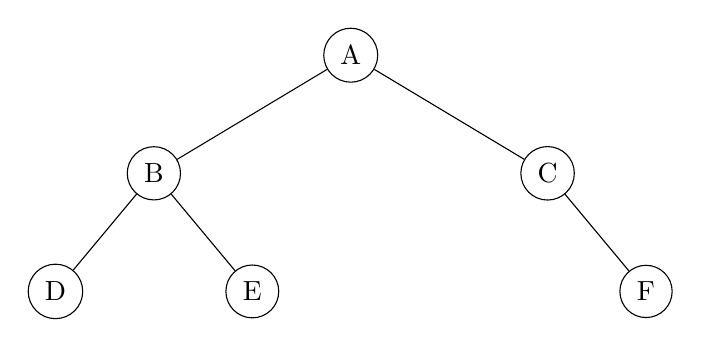
\begin{tikzpicture}[
    every node/.style = {minimum width=1.5em, draw, circle},
    level/.style = {sibling distance = 5cm/#1, level distance = 1.5cm}
  ]
  \node {A}
  child { node {B}
    child { node {D} }
    child { node {E} }
  }
  child { node {C}
    child[missing]
    child { node {F} }
  };
\end{tikzpicture}
\caption{二叉树示例}
\end{figure}

\subsubsection{二叉树的存储结构}

\paragraph{顺序存储} 适用于完全二叉树,使用数组存储,按层序编号。
\begin{itemize}
\item 若某结点的下标为 $i$,则其左孩子下标为 $2i$,右孩子下标为 $2i+1$
\item 若某结点的下标为 $i$,则其双亲结点下标为 $\lfloor i/2 \rfloor$
\end{itemize}

\paragraph{链式存储} 使用二叉链表,每个结点包含数据域和左右指针域。
\begin{lstlisting}[language=C]
typedef struct BiNode {
    ElemType data;           // 数据域
    struct BiNode *lchild;   // 左孩子指针
    struct BiNode *rchild;   // 右孩子指针
} BiNode, *BiTree;
\end{lstlisting}

\subsection{二叉树的遍历}

\subsubsection{先序遍历}
\textcolor{red}{先序遍历(Preorder Traversal)的访问顺序:根结点 $\rightarrow$ 左子树 $\rightarrow$ 右子树}

\begin{algorithm}
\caption{先序遍历算法}
\begin{algorithmic}[1]
  \Procedure{PreOrder}{$T$}
  \If{$T \neq NULL$}
  \State Visit($T$)          \Comment{访问根结点}
  \State PreOrder($T$.lchild) \Comment{先序遍历左子树}
  \State PreOrder($T$.rchild) \Comment{先序遍历右子树}
  \EndIf
  \EndProcedure
\end{algorithmic}
\end{algorithm}

\subsubsection{中序遍历}
\textcolor{red}{中序遍历(Inorder Traversal)的访问顺序:左子树 $\rightarrow$ 根结点 $\rightarrow$ 右子树}

\begin{algorithm}
\caption{中序遍历算法}
\begin{algorithmic}[1]
  \Procedure{InOrder}{$T$}
  \If{$T \neq NULL$}
  \State InOrder($T$.lchild)  \Comment{中序遍历左子树}
  \State Visit($T$)           \Comment{访问根结点}
  \State InOrder($T$.rchild)  \Comment{中序遍历右子树}
  \EndIf
  \EndProcedure
\end{algorithmic}
\end{algorithm}

\subsubsection{后序遍历}
\textcolor{red}{后序遍历(Postorder Traversal)的访问顺序:左子树 $\rightarrow$ 右子树 $\rightarrow$ 根结点}

\begin{algorithm}
\caption{后序遍历算法}
\begin{algorithmic}[1]
  \Procedure{PostOrder}{$T$}
  \If{$T \neq NULL$}
  \State PostOrder($T$.lchild) \Comment{后序遍历左子树}
  \State PostOrder($T$.rchild) \Comment{后序遍历右子树}
  \State Visit($T$)            \Comment{访问根结点}
  \EndIf
  \EndProcedure
\end{algorithmic}
\end{algorithm}

\subsubsection{层序遍历}
\textcolor{red}{层序遍历(Level Order Traversal)的访问顺序:从上到下、从左到右,逐层访问树中的结点。}

\begin{algorithm}
\caption{层序遍历算法}
\begin{algorithmic}[1]
  \Procedure{LevelOrder}{$T$}
  \State 初始化队列 $Q$
  \If{$T \neq NULL$}
  \State 将根结点 $T$ 入队
  \While{队列 $Q$ 非空}
  \State 出队一个结点 $p$
  \State Visit($p$)
  \If{$p$.lchild $\neq$ NULL}
  \State 将 $p$.lchild 入队
  \EndIf
  \If{$p$.rchild $\neq$ NULL}
  \State 将 $p$.rchild 入队
  \EndIf
  \EndWhile
  \EndIf
  \EndProcedure
\end{algorithmic}
\end{algorithm}

\subsection{线索二叉树}

\subsubsection{概念}
\textcolor{red}{线索二叉树(Threaded Binary Tree)是一种利用二叉树中空指针域的存储结构,通过这些空指针域存放指向前驱或后继的指针(称为线索)。}

\subsubsection{类型}
\begin{itemize}
\item \textbf{前序线索二叉树}:按照前序遍历建立线索
\item \textbf{中序线索二叉树}:按照中序遍历建立线索
\item \textbf{后序线索二叉树}:按照后序遍历建立线索
\end{itemize}

\subsubsection{存储结构}
\begin{lstlisting}[language=C]
typedef struct ThreadNode {
    ElemType data;
    struct ThreadNode *lchild, *rchild;
    int ltag, rtag;  // 标志位,0表示孩子,1表示线索
} ThreadNode, *ThreadTree;
\end{lstlisting}

\begin{figure}[h]
\centering
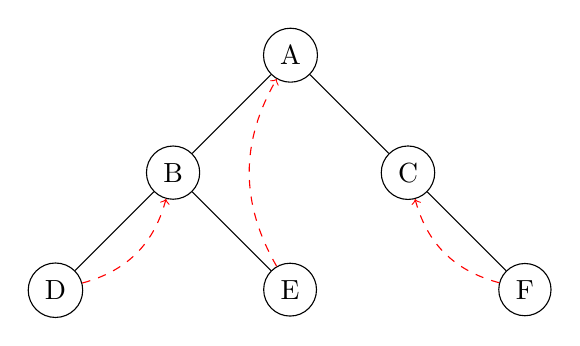
\begin{tikzpicture}[
    every node/.style = {minimum width=1.5em, draw, circle},
    level/.style = {sibling distance = 5cm/#1, level distance = 1.5cm}
  ]
  \node (a) {A};
  \node (b) [below left=of a] {B};
  \node (c) [below right=of a] {C};
  \node (d) [below left=of b] {D};
  \node (e) [below right=of b] {E};
  \node (f) [below right=of c] {F};

  \draw (a) -- (b);
  \draw (a) -- (c);
  \draw (b) -- (d);
  \draw (b) -- (e);
  \draw (c) -- (f);

  \draw[->,dashed,red] (d) to[bend right] (b);
  \draw[->,dashed,red] (e) to[bend left] (a);
  \draw[->,dashed,red] (f) to[bend left] (c);
\end{tikzpicture}
\caption{中序线索二叉树示例(红色虚线表示线索)}
\end{figure}

\subsection{哈夫曼树}

\subsubsection{概念}
\textcolor{red}{哈夫曼树(Huffman Tree),也称为最优二叉树,是一种带权路径长度最小的二叉树。其中,树的带权路径长度为从树根到每个叶子结点的路径长度乘以该结点权值之和。}

\subsubsection{构造算法}
\begin{algorithm}
\caption{哈夫曼树构造算法}
\begin{algorithmic}[1]
  \Procedure{HuffmanTree}{$w[1...n]$}  \Comment{$w[1...n]$为n个权值}
  \State 初始化:将n个权值分别作为n棵仅含一个结点的二叉树
  \For{$i = 1$ to $n-1$}
  \State 在森林中选取两棵根结点权值最小的树,分别记为 $T_1$ 和 $T_2$
  \State 构造一棵新的二叉树 $T$,根结点权值为 $T_1$ 和 $T_2$ 的权值之和
  \State 分别以 $T_1$ 和 $T_2$ 作为新二叉树 $T$ 的左、右子树
  \State 从森林中删除 $T_1$ 和 $T_2$,将新树 $T$ 加入森林
  \EndFor
  \State \Return 森林中唯一的树(即哈夫曼树)
  \EndProcedure
\end{algorithmic}
\end{algorithm}

\begin{example}
已知权值集合 $\{7, 5, 2, 4\}$,构造哈夫曼树。

\begin{figure}[h]
  \centering
  \begin{tikzpicture}[
      every node/.style = {minimum width=2em, draw, circle},
      level/.style = {sibling distance = 5cm/#1, level distance = 1.5cm}
    ]
    \node {18}
    child { node {7} }
    child { node {11}
      child { node {5} }
      child { node {6}
        child { node {2} }
        child { node {4} }
      }
    };
  \end{tikzpicture}
  \caption{构造的哈夫曼树}
\end{figure}

带权路径长度 WPL = $7 \times 1 + 5 \times 2 + 2 \times 3 + 4 \times 3 = 7 + 10 + 6 + 12 = 35$
\end{example}

\subsubsection{哈夫曼编码}
哈夫曼编码是一种基于哈夫曼树的前缀编码,常用于数据压缩。其特点是:

\begin{itemize}
\item 频率高的字符编码短,频率低的字符编码长
\item 没有任何一个字符的编码是另一个字符编码的前缀
\end{itemize}

\begin{example}
对于字符集 \{A, B, C, D\} 和对应频率 \{7, 5, 2, 4\},基于上面构造的哈夫曼树,可得编码:
\begin{itemize}
  \item A:0(频率最高,编码最短)
  \item B:10
  \item C:110
  \item D:111
\end{itemize}
\end{example}

\subsection{二叉排序树}

\textcolor{red}{二叉排序树(Binary Search Tree, BST)是一种特殊的二叉树,具有以下性质:}
\begin{itemize}
\item 左子树上所有结点的值均小于根结点的值
\item 右子树上所有结点的值均大于根结点的值
\item 左右子树也分别是二叉排序树
\end{itemize}

\subsubsection{基本操作}
\begin{itemize}
\item \textbf{查找}:从根结点开始,若目标值小于当前结点则向左子树查找,大于则向右子树查找
\item \textbf{插入}:类似查找过程,找到应插入的位置后创建新结点
\item \textbf{删除}:分三种情况:删除叶结点、删除只有一个子树的结点、删除有两个子树的结点
\end{itemize}

\subsection{平衡二叉树}

\textcolor{red}{平衡二叉树(Balanced Binary Tree)是一种特殊的二叉排序树,其任意结点的左右子树高度差不超过1。}

\subsubsection{平衡因子}
结点的平衡因子(Balance Factor)定义为左子树高度减去右子树高度。平衡二叉树中所有结点的平衡因子只能是-1、0或1。

\subsubsection{AVL树的旋转操作}
不平衡情况分为四种:
\begin{itemize}
\item \textbf{LL型}:在结点的左孩子的左子树上插入导致不平衡,需右旋
\item \textbf{RR型}:在结点的右孩子的右子树上插入导致不平衡,需左旋
\item \textbf{LR型}:在结点的左孩子的右子树上插入导致不平衡,需先左旋后右旋
\item \textbf{RL型}:在结点的右孩子的左子树上插入导致不平衡,需先右旋后左旋
\end{itemize}

\section{图}

\subsection{图的基本概念}

\subsubsection{定义}
\textcolor{red}{图(Graph)是由顶点集合 V 和边集合 E 组成的二元组 G = (V, E),其中每条边连接一对顶点。}

\subsubsection{基本术语}
\begin{itemize}
\item \textbf{有向图}:边有方向,称为弧(Arc)。弧的起点称为弧尾,终点称为弧头
\item \textbf{无向图}:边无方向,用无序对 (v, w) 表示
\item \textbf{完全图}:任意两个顶点之间都有边相连的图
  \begin{itemize}
    \item 有 n 个顶点的无向完全图有 $\frac{n(n-1)}{2}$ 条边
    \item 有 n 个顶点的有向完全图有 $n(n-1)$ 条弧
  \end{itemize}
\item \textbf{权}:边或弧上的数值,表示从一个顶点到另一个顶点的距离或代价
\item \textbf{子图}:原图中部分顶点及相连边构成的图
\end{itemize}

\subsubsection{顶点与边的关系}
\begin{itemize}
\item \textbf{顶点的度}:与该顶点相连的边的条数
  \begin{itemize}
    \item 在有向图中分为入度(入边数)和出度(出边数)
    \item 顶点的度 = 入度 + 出度
  \end{itemize}
\item \textbf{路径}:从一个顶点到另一个顶点经过的顶点序列
\item \textbf{路径长度}:路径上边或弧的数目或权值之和
\item \textbf{回路/环}:起点和终点相同的路径
\item \textbf{简单路径}:除起点和终点可以相同外,其余顶点均不相同的路径
\item \textbf{连通}:两个顶点之间存在路径
\end{itemize}

\subsubsection{特殊图}
\begin{itemize}
\item \textbf{连通图}:任意两个顶点都是连通的无向图
\item \textbf{连通分量}:无向图中的极大连通子图
\item \textbf{强连通图}:任意两个顶点都互相可达的有向图
\item \textbf{强连通分量}:有向图中的极大强连通子图
\item \textbf{生成树}:包含图中全部顶点的一个极小连通子图
\item \textbf{生成森林}:非连通图的各个连通分量的生成树的集合
\end{itemize}

\begin{figure}[h]
\centering
\begin{tikzpicture}[
    every node/.style = {minimum width=1.5em, draw, circle},
    >=stealth
  ]
  % 无向图
  \begin{scope}[shift={(-4,0)}]
    \node (a1) at (0,2) {A};
    \node (b1) at (2,2) {B};
    \node (c1) at (0,0) {C};
    \node (d1) at (2,0) {D};
    \draw (a1) -- (b1);
    \draw (a1) -- (c1);
    \draw (b1) -- (d1);
    \draw (c1) -- (d1);
    \node[draw=none] at (1,-1) {无向图};
  \end{scope}

  % 有向图
  \begin{scope}[shift={(2,0)}]
    \node (a2) at (0,2) {A};
    \node (b2) at (2,2) {B};
    \node (c2) at (0,0) {C};
    \node (d2) at (2,0) {D};
    \draw[->] (a2) -- (b2);
    \draw[->] (a2) -- (c2);
    \draw[->] (b2) -- (d2);
    \draw[->] (c2) -- (d2);
    \node[draw=none] at (1,-1) {有向图};
  \end{scope}
\end{tikzpicture}
\caption{无向图和有向图示例}
\end{figure}

\subsection{图的存储结构}

\subsubsection{邻接矩阵}

\textcolor{red}{邻接矩阵(Adjacency Matrix)是一种使用二维数组存储图的方法,用于表示顶点之间的相邻关系。}

\begin{itemize}
\item \textbf{无向图}:$A[i][j] = A[j][i]$(矩阵对称),值为边的权值或1(表示有边)
\item \textbf{有向图}:$A[i][j]$ 表示从顶点 $i$ 到顶点 $j$ 的弧
\item \textbf{稠密图}适合用邻接矩阵表示
\end{itemize}

\begin{lstlisting}[language=C]
#define MaxVertexNum 100  // 最大顶点数
typedef struct {
    char Vex[MaxVertexNum];           // 顶点表
    int Edge[MaxVertexNum][MaxVertexNum];  // 邻接矩阵
    int vexnum, arcnum;               // 顶点数和弧数
} MGraph;
\end{lstlisting}

\subsubsection{邻接表}

\textcolor{red}{邻接表(Adjacency List)是一种链式存储结构,每个顶点对应一个单链表,链表中的结点表示该顶点的所有邻接顶点。}

\begin{itemize}
\item 适合存储稀疏图
\item 容易找到给定顶点的所有邻接点
\item 判断两个顶点是否相邻需要搜索
\end{itemize}

\begin{lstlisting}[language=C]
typedef struct ArcNode {      // 边表结点
    int adjvex;               // 该弧所指向的顶点的位置
    struct ArcNode *next;     // 指向下一条弧的指针
    // InfoType info;         // 网的权值
} ArcNode;

typedef struct VNode {        // 顶点表结点
    VertexType data;          // 顶点信息
    ArcNode *first;           // 指向第一条依附该顶点的弧
} VNode, AdjList[MaxVertexNum];

typedef struct {
    AdjList vertices;         // 邻接表
    int vexnum, arcnum;       // 顶点数和弧数
} ALGraph;
\end{lstlisting}

\begin{figure}[h]
\centering
\begin{tikzpicture}[
    node distance=0.5cm and 1cm,
    vnode/.style={draw, rectangle, minimum width=1cm, minimum height=0.6cm},
    arcnode/.style={draw, rectangle, minimum width=1.5cm, minimum height=0.6cm}
  ]

  % 示例图
  \begin{scope}[shift={(0,2)}]
    \node[draw, circle] (a) at (0,0) {A};
    \node[draw, circle] (b) at (2,0) {B};
    \node[draw, circle] (c) at (0,-1.5) {C};
    \node[draw, circle] (d) at (2,-1.5) {D};

    \draw (a) -- (b);
    \draw (a) -- (c);
    \draw (b) -- (c);
    \draw (c) -- (d);

    \node[draw=none] at (1,-2) {图};
  \end{scope}

  % 邻接表表示
  \begin{scope}[shift={(0,-2)}]
    \node[vnode] (va) at (0,0) {A};
    \node[arcnode] (ab) at (1.5,0) {B};
    \node[arcnode] (ac) at (3,0) {C};
    \node[arcnode] (anull) at (4.5,0) {NULL};

    \node[vnode] (vb) at (0,-1) {B};
    \node[arcnode] (ba) at (1.5,-1) {A};
    \node[arcnode] (bc) at (3,-1) {C};
    \node[arcnode] (bnull) at (4.5,-1) {NULL};

    \node[vnode] (vc) at (0,-2) {C};
    \node[arcnode] (ca) at (1.5,-2) {A};
    \node[arcnode] (cb) at (3,-2) {B};
    \node[arcnode] (cd) at (4.5,-2) {D};
    \node[arcnode] (cnull) at (6,-2) {NULL};

    \node[vnode] (vd) at (0,-3) {D};
    \node[arcnode] (dc) at (1.5,-3) {C};
    \node[arcnode] (dnull) at (3,-3) {NULL};

    \draw[->] (va) -- (ab);
    \draw[->] (ab) -- (ac);
    \draw[->] (ac) -- (anull);

    \draw[->] (vb) -- (ba);
    \draw[->] (ba) -- (bc);
    \draw[->] (bc) -- (bnull);

    \draw[->] (vc) -- (ca);
    \draw[->] (ca) -- (cb);
    \draw[->] (cb) -- (cd);
    \draw[->] (cd) -- (cnull);

    \draw[->] (vd) -- (dc);
    \draw[->] (dc) -- (dnull);

    \node[draw=none] at (3,-3.7) {邻接表};
  \end{scope}
\end{tikzpicture}
\caption{邻接表示例}
\end{figure}

\subsection{图的遍历算法}

\subsubsection{广度优先搜索 (BFS)}

\textcolor{red}{广度优先搜索(Breadth-First Search)类似于树的层序遍历,按照距离起始顶点由近到远的顺序访问图中的顶点。}

\begin{algorithm}
\caption{广度优先搜索算法}
\begin{algorithmic}[1]
  \Procedure{BFS}{$G, start$}
  \State 初始化访问标记数组 visited[G.vexnum] = \{FALSE\}
  \State 初始化队列 Q
  \State 访问起始顶点 start
  \State visited[start] = TRUE
  \State 将 start 入队列 Q
  \While{队列 Q 非空}
  \State 出队一个顶点 v
  \For{顶点 v 的每个邻接点 w}
  \If{visited[w] == FALSE}
  \State 访问顶点 w
  \State visited[w] = TRUE
  \State 将 w 入队列 Q
  \EndIf
  \EndFor
  \EndWhile
  \EndProcedure
\end{algorithmic}
\end{algorithm}

\paragraph{BFS性质}
\begin{itemize}
\item 时间复杂度:邻接矩阵为 $O(|V|^2)$,邻接表为 $O(|V|+|E|)$
\item 空间复杂度:$O(|V|)$
\item 能够求解无权图的单源最短路径问题
\end{itemize}

\subsubsection{深度优先搜索 (DFS)}

\textcolor{red}{深度优先搜索(Depth-First Search)类似于树的先序遍历,沿着一条路径一直走到底,直到不能再继续为止,然后回溯选择其他路径。}

\begin{algorithm}
\caption{深度优先搜索算法}
\begin{algorithmic}[1]
  \Procedure{DFS}{$G, v$}
  \State 访问顶点 v
  \State visited[v] = TRUE
  \For{顶点 v 的每个邻接点 w}
  \If{visited[w] == FALSE}
  \State DFS($G, w$)
  \EndIf
  \EndFor
  \EndProcedure
\end{algorithmic}
\end{algorithm}

\paragraph{DFS性质}
\begin{itemize}
\item 时间复杂度:邻接矩阵为 $O(|V|^2)$,邻接表为 $O(|V|+|E|)$
\item 空间复杂度:最坏情况 $O(|V|)$(递归栈深度)
\end{itemize}

\subsection{最小生成树}

\textcolor{red}{最小生成树(Minimum Spanning Tree,MST)是一副连通加权无向图中一棵权值最小的生成树。}

\subsubsection{Prim算法}

Prim 算法从单一顶点开始,逐步将新顶点纳入到生成树中,每次选择代价最小的边。

\begin{algorithm}
\caption{Prim算法}
\begin{algorithmic}[1]
  \Procedure{Prim}{$G, start$}
  \State 初始化集合 $U = \{start\}$,表示已加入生成树的顶点集合
  \State 初始化集合 $V-U$,表示尚未加入生成树的顶点集合
  \While{$U \neq V$}
  \State 在所有连接 $U$ 和 $V-U$ 的边中,找到权值最小的边 $(u,v)$,其中 $u \in U$,$v \in V-U$
  \State 将顶点 $v$ 加入集合 $U$
  \State 将边 $(u,v)$ 加入最小生成树
  \EndWhile
  \EndProcedure
\end{algorithmic}
\end{algorithm}

\paragraph{Prim算法性质}
\begin{itemize}
\item 时间复杂度:$O(|V|^2)$(邻接矩阵),可优化到 $O(|E|\log|V|)$(优先队列)
\item 适合于稠密图
\end{itemize}

\subsubsection{Kruskal算法}

Kruskal 算法按照边的权值从小到大依次选择边,保证不形成环。

\begin{algorithm}
\caption{Kruskal算法}
\begin{algorithmic}[1]
  \Procedure{Kruskal}{$G$}
  \State 初始化最小生成树 $T$ 为空
  \State 将图 $G$ 中的边按权值从小到大排序
  \For{图 $G$ 中每条边 $(u,v)$(按权值从小到大)}
  \If{加入边 $(u,v)$ 不会在 $T$ 中形成环}
  \State 将边 $(u,v)$ 加入 $T$
  \EndIf
  \EndFor
  \EndProcedure
\end{algorithmic}
\end{algorithm}

\paragraph{Kruskal算法性质}
\begin{itemize}
\item 时间复杂度:$O(|E|\log|E|)$
\item 适合于稀疏图
\end{itemize}

\begin{figure}[h]
\centering
\begin{tikzpicture}[
    every node/.style = {minimum width=1.5em, draw, circle},
    >=stealth
  ]
  % 原图
  \begin{scope}[shift={(0,0)}]
    \node (a) at (0,2) {A};
    \node (b) at (2,2) {B};
    \node (c) at (0,0) {C};
    \node (d) at (2,0) {D};
    \draw (a) -- node[draw=none, fill=white] {2} (b);
    \draw (a) -- node[draw=none, fill=white] {6} (c);
    \draw (b) -- node[draw=none, fill=white] {3} (d);
    \draw (c) -- node[draw=none, fill=white] {4} (d);
    \draw (b) -- node[draw=none, fill=white] {5} (c);
    \node[draw=none] at (1,-1) {带权图};
  \end{scope}

  % 最小生成树
  \begin{scope}[shift={(6,0)}]
    \node (a) at (0,2) {A};
    \node (b) at (2,2) {B};
    \node (c) at (0,0) {C};
    \node (d) at (2,0) {D};
    \draw[red, thick] (a) -- node[draw=none, fill=white] {2} (b);
    \draw[red, thick] (b) -- node[draw=none, fill=white] {3} (d);
    \draw[red, thick] (c) -- node[draw=none, fill=white] {4} (d);
    \node[draw=none] at (1,-1) {最小生成树};
  \end{scope}
\end{tikzpicture}
\caption{最小生成树示例}
\end{figure}

\subsection{最短路径}

\subsubsection{Dijkstra算法}

\textcolor{red}{Dijkstra算法用于计算一个顶点到其他所有顶点的最短路径,适用于所有边权值为非负数的图。}

\begin{algorithm}
\caption{Dijkstra算法}
\begin{algorithmic}[1]
  \Procedure{Dijkstra}{$G, start$}
  \State 初始化距离数组 $dist[i] = \infty$,$dist[start] = 0$
  \State 初始化前驱数组 $path[i] = -1$
  \State 初始化集合 $S = \emptyset$,表示已确定最短路径的顶点集合
  \While{$S$ 不包含所有顶点}
  \State 在 $V-S$ 中选择距离最小的顶点 $u$
  \State 将 $u$ 加入集合 $S$
  \For{顶点 $u$ 的每个邻接点 $v$}
  \If{$dist[u] + weight(u,v) < dist[v]$}
  \State $dist[v] = dist[u] + weight(u,v)$
  \State $path[v] = u$
  \EndIf
  \EndFor
  \EndWhile
  \State \Return $dist, path$
  \EndProcedure
\end{algorithmic}
\end{algorithm}

\paragraph{Dijkstra算法性质}
\begin{itemize}
\item 时间复杂度:$O(|V|^2)$(邻接矩阵),可优化到 $O(|E|\log|V|)$(优先队列)
\item 不适用于有负权边的图
\end{itemize}

\begin{figure}[h]
\centering
\begin{tikzpicture}[
    every node/.style = {minimum width=1.5em, draw, circle},
    >=stealth
  ]
  % 原图
  \begin{scope}[shift={(0,0)}]
    \node (a) at (0,2) {A};
    \node (b) at (2,2) {B};
    \node (c) at (0,0) {C};
    \node (d) at (2,0) {D};
    \draw[->] (a) -- node[draw=none, fill=white] {2} (b);
    \draw[->] (a) -- node[draw=none, fill=white] {6} (c);
    \draw[->] (b) -- node[draw=none, fill=white] {3} (d);
    \draw[->] (c) -- node[draw=none, fill=white] {1} (d);
    \draw[->] (b) -- node[draw=none, fill=white] {1} (c);
  \end{scope}

  % 最短路径
  \begin{scope}[shift={(6,0)}]
    \node (a) at (0,2) {A};
    \node (b) at (2,2) {B};
    \node (c) at (0,0) {C};
    \node (d) at (2,0) {D};
    \draw[->, red, thick] (a) -- node[draw=none, fill=white] {2} (b);
    \draw[->, red, thick] (b) -- node[draw=none, fill=white] {1} (c);
    \draw[->, red, thick] (c) -- node[draw=none, fill=white] {1} (d);
    \node[draw=none] at (1,-1) {从A到D的最短路径};
  \end{scope}
\end{tikzpicture}
\caption{Dijkstra最短路径示例}
\end{figure}

\subsubsection{Floyd算法}

\textcolor{red}{Floyd算法是一种动态规划算法,用于寻找加权图中所有顶点之间的最短路径。}

\begin{algorithm}
\caption{Floyd算法}
\begin{algorithmic}[1]
  \Procedure{Floyd}{$G$}
  \State 初始化距离矩阵 $D[i][j] = G.Edge[i][j]$
  \State 初始化路径矩阵 $Path[i][j] = j$(若 $i$ 到 $j$ 有直接路径)
  \For{$k = 0$ to $n-1$} \Comment{以 $k$ 为中转点}
  \For{$i = 0$ to $n-1$}
  \For{$j = 0$ to $n-1$}
  \If{$D[i][k] + D[k][j] < D[i][j]$}
  \State $D[i][j] = D[i][k] + D[k][j]$
  \State $Path[i][j] = Path[i][k]$
  \EndIf
  \EndFor
  \EndFor
  \EndFor
  \EndProcedure
\end{algorithmic}
\end{algorithm}

\paragraph{Floyd算法性质}
\begin{itemize}
\item 时间复杂度:$O(|V|^3)$
\item 空间复杂度:$O(|V|^2)$
\item 可处理有负权边的图,但不能有负权回路
\end{itemize}

\end{document}